% Please use the skeleton file you have received in the
% invitation-to-submit email, where your data are already
% filled in. Otherwise please make sure you insert your
% data according to the instructions in PoSauthmanual.pdf
\documentclass{PoS}

\title{Containerization of CMS Applications with Docker}

\ShortTitle{Containerization of CMS Applications with Docker}

\author{Giulio Eulisse\\
        CERN\\
        E-mail: \email{Giulio.Eulisse@cern.ch}}

\author{Tommaso Boccali\\
        INFN-Pisa\\
        E-mail: \email{Tommaso.Boccali@pi.infn.it}}

\author{Enrico Mazzoni\\
        INFN-Pisa\\
        E-mail: \email{enrico.mazzoni@pi.infn.it}}

\author{\speaker{Daniele Bonacorsi}\\
        University of Bologna and INFN-Bologna, Italy\\
        E-mail: \email{daniele.bonacorsi@unibo.it}}


\abstract{Clouds and virtualisation offer typical answers to the needs of large-scale computing centres to satisfy diverse sets of user communities in terms of architecture, OS, etc. On the other hand, solutions like Docker seems to emerge as a way to rely on Linux kernel capabilities to package only the applications and the development environment needed by the users, thus solving several resource management issues related to cloud-like solutions. In this paper, an exploratory work done based on the workflows of the CMS experiment at the LHC accelerator at CERN is presented. Progresses towards the deployment of a full data center via exploiting \emph{container-ised} software stacks for CMS will be reported and discussed.}

\FullConference{International Symposium on Grids and Clouds (ISGC) 2015,\\
                15 -20 March 2015\\
                Academia Sinica, Taipei, Taiwan}


\begin{document}

\section{Introduction}

Docker~\cite{docker} is an open platform to build, ship and run distributed applications. It is a container-based virtualisation framework that uses Linux containers (LXC) as the core technology, with a large set of tools allowing for large scale container handling, shipping and deployment. It allows for easy container contextualization, and for inter-container communications. Docker utilisation is becoming the de-facto standard for container based virtualisation, and is the recommended solution endorsed by most heavy weight IT providers. Some examples are Spotify, that uses Docker for continuous delivery, service testing and deployment; Baidu, that uses Docker as a Platform-as-a-Service (PaaS), profiting of its flexibility for many framework and applications; eBay, that uses Docker for its easy application deployment, and for continuous integration process; and many more. Recently, Docker has reached 120k lines of code, about 10k commits and roughy 600 core contributors, of which about 95\% work outside Docker.

\section{Docker as a tool for light virtualisation}

Virtualisation can be achieved in several ways, depending on the desired (or acceptable) level of invasiveness. Setting aside solutions when the whole system hardware is emulated (like QEMU), the industry reference technologies are full system virtualisation (OpenStack~\cite{openstack}, OpenNebula~\cite{opennebula}), where each virtualised machine has its own running kernel, and kernel based process isolation, which has been a possibility in Linux since the beginning, via \emph{chroot}, and more recently via \emph{c-groups} and projects like the Linux Container (\emph{LXC}~\cite{lxc}). The former technology has a broader scope, being able to utilize different operating systems on the same physical host (e.g. mixing Windows and Linux machines), but pays a price in terms of resource utilisation (mainly RAM, to a smaller extent CPU reduced efficiency) and access to high performance devices; it is considered an overkill in our field, where more or less all the scientific computation are carried out on Linux machines. Linux Containers, at the heart of the Docker technology, instead of simulating complete machines, just provede process separation and sand-boxing over a common kernel all the machines share. This is particularly adequate in an environment where system standardisation has already been achieved to a large extent, for example by the adoption of WLCG-provided Middleware.
Docker provides CPU, memory and filesystem isolation, and can run different processes on the same kernel but with completely different runtime (e.g. one can run SLC5 on SLC6 or on Ubuntu).

Docker adds on top of LXC a complete series of tools for image storing, deployment, testing and contextualization, as well as for container handling (start/stop/...) and communications; derived images can be based on exiting images, with Docker taking care to save only the deltas between them. It also add a public repository (Docker Hub, {\verb hub.docker.com}), which allows for safe image storing and easy deployment for open software projects, which provides already cooked images for most of the widespread linux based operating systems.

Currently Docker Hub hosts  ~45k publicly accessible images, and starting a new container on a linux based machine is as easy as a single line command:
%
\begin{verbatim}
        $ docker run -it centos:centos7 cat /etc/redhat-release
        CentOS Linux release 7.0.1406 (Core)
\end{verbatim}
%
The images can be built using so called ``Dockerfiles'', e.g.:
%
\begin{verbatim}
FROM cmssw/slc6-vanilla
    RUN yum -y update && yum -y install rubygems ruby-devel \
                                      gcc ruby193
    RUN echo "gem: --no-ri --no-rdoc" > ~/.gemrc && \
        gem install puppet && \
        gem install librarian-puppet -v 1.0.9
    CMD /bin/bash
\end{verbatim}
%
All images are layered, there is no need to re-download previously downloaded layers (e.g. each of the above statements is a layer). Several CMS examples are documented~\cite{DockerGiulio}.

Additionally, it is relatively straightforward to set-up Docker on one's own operating system of choice. Docker comes pre-packaged on most modern distributions, including slc6:
%
\begin{verbatim}
    sudo yum install docker-io
    sudo service docker start
\end{verbatim}
%
The test set-up (used for most tests reported in this paper) consists of 2 socket Intel(R) Xeon(R) CPU E5-2630L 0 \@ 2.00GHz (12 real cores, 24 with HT); 2 GHz, 16 MB Cache, Rotating disks; Real HW, no hypervisor, Docker running directly on top of slc6. On the other hand, for Mac/Windows users an interesting option is boot2docker.io: it provides a VirtualBox environment and wrappers which make it look like a native setup. A lightweight Linux distribution based on Tiny Core Linux made specifically to run Docker containers is used; it runs completely from RAM, weighs ~27MB and boots in few seconds.

\section{Examples of CMS applications}

As stated in the previous section, several CMS examples are documented~\cite{DockerGiulio}. One of these is particularly interesting and will be discussed briefly. ``ParFullCMS''~\cite{parfullcms} is a parametrised Geant4-based geometric description of the CMS detector. It is mainly used for benchmarking (e.g. it is being used to do realistic tests of CMS software on ARM). It can be installed from the CMS apt repository, and running it is as easy as:
%
\begin{verbatim}
    docker run -e EVENTS=2400 -v $PWD:/data -it cmssw/parfullcms
\end{verbatim}
%
One can easily configure the number of events and the number of threads to use, and can run Geant4 simulation. Several tests done with ParFullCMS (3 runs, 2400 evts, 24 threads) with Docker and on bare metal show that the time performances are comparable, the confirming that no overhead is observed when using Docker.

Another interesting example is that one can ship the entire CMS software (CMSSW) as a whole to the host i.e. not downloading it via CVMFS, but just ship it all from the outside. This may become interesting to be exploited in case one wants to run a set of CMS specific tests which are usually run for CMS releases validation, e.g.:
%
\begin{verbatim}
    docker run -e WORKFLOW=25.0 -it cmssw/cmssw:CMSSW_7_3_0
\end{verbatim}
%
Suppose e.g. that one has a brand new machine, and wants to know how fast it is for CMS workflows. It is sufficient to put (roughly) about 10 GB on a USB key and run a real CMSSW workflow and measure (10 GB correspond to a release plus the necessary input files to be shipped - any limit in the shipped size that Docker does not support out of the box can be overcome by starting it with particular options). This has been tested with a CMS reconstruction workflow (ttbar sample), and it was observed that bare metal vs Docker
times are very similar, basically indistinguishable.

This opens the door to interesting application in terms of benchmarking. After SPEC and SPECfp, it was soon realised that standard benchmarking was not really adequate for HEP, as a machine benchmarked as 2x was not twice as fast for LHC typical applications (which are quite RAM-intensive, heavy on caches, etc). HepSpec06 was hence designed in 2006 to scale as typical LHC experiments applications. Today, this is not completely true anymore, especially in moving to 64-bit. Docker (see previous example), might hence be the tool to offer a simple, portable way to run a benchmark. And this could be given to hardware vendors to run realistic (and a large set, and always up-to-date) benchmarks of CMS workflows.

\section{``Dockerizing'' a computing site}
Virtualisation technologies are the best choice when dealing when dealing with users with diverse needs in term of computing resources. While Linux is the de-facto standard for most scientific uses, precise hardware and software needs can still vary to the extent of not allowing for a catch-all solution. Software from previous generation experiment is often not validated for the latest-greatest Linux versions, for example, and thus cannot coexist with recent experiments which instead prefer the best performance coming with newer releases.

The CMS Pisa Tier-2 center is one of the biggest Italian scientific computing center: it is a Tier-2 in WLCG, supporting CMS, but CMS is actually a minority part of the resources/users, which include also LHCb and ATLAS, 20 more Virtual Organizations, a National Theoretical Physics computing center, a 2000 (and more) cores fluidodynamic cluster (used in industry related researches). In terms of resources it consists of ~8k cores, >2 PB, highly heterogeneous WN hosts (some are 1 Gbe, some 10 Gbe, some Infiniband). Also the OS requests are heterogeneous (some still SL5, even SL4 up to some months ago; some prefer very recent releases, generally OpenSuSe). The only common points between such a diverse user-community are: 

\begin{itemize}
\item GPFS~\cite{gpfs} is used to serve data for all the use-cases supported on-site;
\item AFS~\cite{afs} is used for user areas; 
\item LSF~\cite{lsf} is used for resource access, also interactive.
\end{itemize}

The main issue in Pisa recently was to understand how to provision the correct environment to all these diverse resources. Virtual Machines (e.g. OpenStack) were considered as an option, but
Pisa also has older machines which are low in RAM. Infiniband connectivity, moreover, seems to loose performance in a completely virtualised environment. The solution identified up to recently so far was a very light virtualisation via chroot. Every host machine (with the very latest OpenSUSE kernel) was starting sand-boxed machines as tar files containing complete SL6 (or SLx) systems,  via chroot. Site-wide file-systems (CVMFS~/cite{cvmfs}/GPFS/AFS~\cite{afs}) were mounted by the host, and then seen by the machines as local file systems using the emph{bind}  tool.
Every machine had pre-installed as many tar files as the possible environments are: these could be un-tarred and ``started'' on demand via a set of scripts, basically forcing the LSF pool the machine lives in. This solution works and it has been in production for Pisa since 3 years.

On the other hand, Docker is to be a viable solution, too. It has the same overhead (virtually 0) as chroot, and comes with the added plus of easier image storing, deployment and control. Basically, three are the main points in favour of Docker adoption in Pisa: 
\begin{itemize}
\item no more tar files and a complicate management;
\item the adoption of a git-like image management, where every action on the repository is properly logged, and you can branch, pull, etc;
\item the very easy deployment of a local image repository, to avoid exposure of sensitive information;
\item the extremely easy conversion of an existing chroot's tar image to a Docker image, via a single command:
\begin{verbatim}
sudo tar -C ExistingChrootBaseDir -c . \
| sudo docker import - PisaWN
\end{verbatim}
\end{itemize}

A Tier-2 on-demand approach was initially planned, where no dependency on the underlying physical architecture was foreseen, but currently it has been decided to privilege ese of deployment and performance over flexibility. Pisa decided hence to mount CVMFS/GPFS/AFS on the host and pass them via ``-v'', instead of relying on the image mounting them via userland tools like Parrot;
The solution also allows for the sharing of CVMFS/AFS caches in case of multiple machines running, and does not force the containers to run in privileged mode, which would not be possible in (e.g.) opportunistic sites.
LSF  runs within the container, and automatically connects the machine to the proper LSF queue, with a start command as follows. all in all, a Worker Node instance is started just via
%
\begin{verbatim}
docker run -v /cvmfs:/cvmfs -v /afs:/afs \
-v /gpfs/ddn:/gpfs/ddn \
-v /chrootlfs/home:/home/grid -d \
-t localregistry.pi.infn.it:5000/enricomazzoni/testwn:0.3 \
/etc/sysconfig/docker-pi/start
\end{verbatim}

The complete workflow of operations is shown if Fig.\ref{fig:dockerPisa}: admin's action selects and starts the appropriate container, which then joins the correct LSF queue and becomes available for processing (via batch system and interactive).

%
Pisa moved ~10\% of the WNs to Docker so far, following an R\&D process of just a couple of weeks. No user actually realised the difference. The rest of the centre will migrate as well in the next few weeks. At this point, the idea would be to move all the services used by CMS via Docker:
\begin{itemize}
\item Squid: just a Linux standard machine;
\item Computing Elements (CEs): one already moved without problems, starting from a chtooed test we had;
\item User Interfacess (UIs): similar to WNs, can share most of their image; 
\item PhEDEx (CMS transfer agents on a User Interfac): a simple modification of the latter;
\item Xrootd redirectors (for CMS data federations): Pisa moved it from chroot and it is already running now with Docker.
\end{itemize}

\section{Conclusions}

In summary, Docker offers interesting opportunities to CMS. It can ship entire CMSSW distributions and do benchmarking easily. It offers plenty of desired features and flexibility at a site level, and all this at no cost in terms of performances (as from the tests done so farm, at least).

The transition in itself is very easy, indeed matter of days, admittedly maybe also because Pisa was already at chroot point - but other works in CMS show that starting from bare metal is as easy,    and Docker provides most of the specific scripts a site may need for image processing, download history, starting, stopping.

In a nutshell, it s a neat tool, and CMS will continue testing it (and possibly integrating it) in its activities.


\begin{figure}
\begin{center}
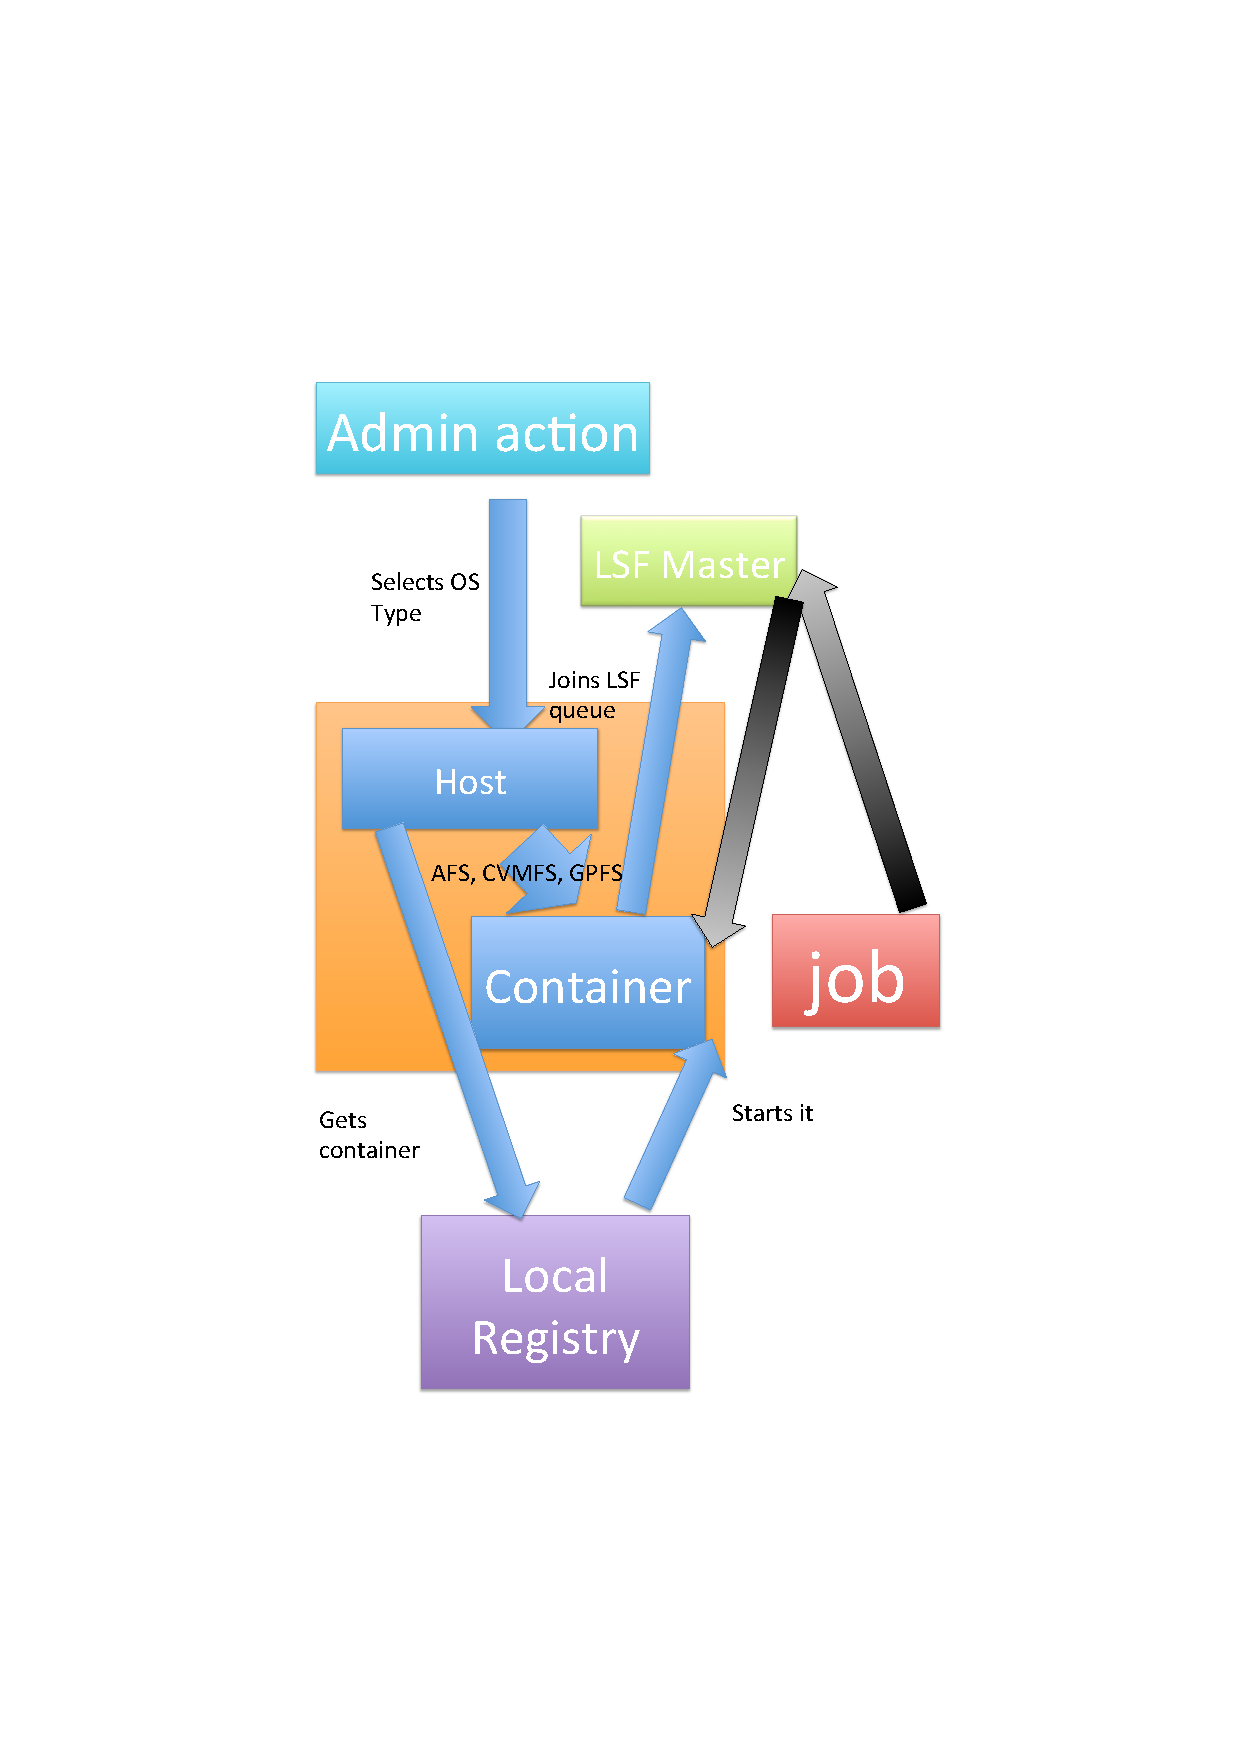
\includegraphics[width=.8\textwidth]{dockerpisa.pdf}
\caption{Workflow from admin's action to a machine accessible via LSF.}
\label{fig:dockerPisa}
\end{center}
\end{figure}
%


\begin{thebibliography}{99}
\bibitem{docker} Docker Web Site, \texttt{http://www.docker.com/}.
\bibitem{openstack}OpenStack, \texttt{https://www.openstack.org/}.
\bibitem{opennebula}OpenNebula, \texttt{http://opennebula.org/}.
\bibitem{lxc}Linux Containers, \texttt{http://en.wikipedia.org/wiki/LXC}.
.\bibitem{gpfs} GPFS: A Shared-Disk File System for Large Computing Clusters, Proceedings of the FAST 2002 Conference on File and Storage Technologies Monterey, California, USA January 28-30, 2002.
\bibitem{afs} OpenAFS, \texttt{http://www.openafs.org/}.
\bibitem{cvmfs} CVMFS, \texttt{http://cernvm.cern.ch/portal/filesystem}.
\bibitem{lsf} LSF, \texttt{http://www-03.ibm.com/systems/platformcomputing/products/lsf}.
\bibitem{parrot}The Parrot Virtual File System, \texttt{The Parrot Virtual File System}.
\bibitem{DockerGiulio} CMS examples with Docker: \texttt{http://github.com/cms-sw/cms-docker}.
\bibitem{parfullcms} ParFullCMS, \texttt{https://github.com/cms-sw/cms-docker/tree/master/parfullcms}.




\end{thebibliography}

\end{document}
